\section{The Symbolic Mirage}
\label{sec:analysis}

\subsection{Symbolic Confirmation Bias}
\label{sec:confirmation-bias}

\looseness=-1 Self-extracted constraints systematically align with the model's majority answer, a persistent empirical property of zero-shot self-extraction pipelines, not a cognitive bias analogy. On Mistral-7B FOLIO, when SICA errs, 83.3\% of constraints support the incorrect answer (bias ratio $4.97\times$; Table~\ref{tab:cross-model-bias}), and 94\% of errors overlap with SC. Z3 rejects only 3.4\% of constraints, and MAX-SAT produces answers identical to count-only aggregation on ${\geq}99\%$ of problems across all weight settings $\alpha$ (Table~\ref{tab:alpha-ablation}), confirming that the formal verification layer is vacuous (Eq.~\ref{eq:degenerate}): 99\% of constraints pass Z3 validation yet add no information beyond majority voting.

\looseness=-1 Crucially, BR $> 1$ is not an independent finding but a corollary of the degeneration identified in Observation~1: under source-attribution scoring, constraint weight is proportional to trace count, so the majority answer necessarily receives more support. A permutation test randomizing constraint--answer associations confirms this ($\text{BR}_\text{excess} \approx 0$, $p > 0.7$; Appendix~\ref{app:constraint-quality}). As a zero-cost diagnostic, BR quantifies the degree of extraction degeneration (how completely constraints collapse to majority-vote equivalents), not an independent theoretical contribution. On problems where SC is correct, constraints still track the majority ($\text{BR}_\text{correct}$ $1.29$--$3.64\times$), confirming that self-extracted constraints reflect distributional frequency rather than logical validity.

\looseness=-1 The pattern generalizes across nine models from 7B to frontier (BR $1.66$--$4.97\times$; Table~\ref{tab:frontier-scb} in Appendix~\ref{app:frontier-scb}) and all eight cells of a $2{\times}2$ generator${\times}$extractor matrix (range $1.94$--$2.70$; Appendix~\ref{app:2x2}). Constraints use trace-specific variables (56.4\% zero variable overlap across answer groups), collapsing aggregation to majority voting.

\looseness=-1 Two controls rule out answer leakage: BR is uniform across reasoning steps (Fisher $p = 0.71$), and removing answer sentences before extraction yields no BR decrease (Wilcoxon $p \geq 0.12$) despite accuracy loss (McNemar $p < 0.013$). The bias reflects a distributional prior embedded throughout reasoning, not answer contamination.

\label{sec:process-kappa}
\looseness=-1 Reasoning-process overlap exceeds answer-level correlation: mean process similarity (pairwise TF-IDF cosine) reaches $0.69$ on Mistral-7B FOLIO, far exceeding answer-level $\kappa$ ($0.41$--$0.51$). The gap generalizes across four families (Table~\ref{tab:cross-model-process}). Under cross-model extraction, SICA gain decreases monotonically with process similarity ($\rho = -1.0$, $p = 0.0083$; Table~\ref{tab:process-gradient}): conditions above process similarity $0.60$ show null gain (Appendix~\ref{app:cil}).

\begin{figure*}[t]
\centering
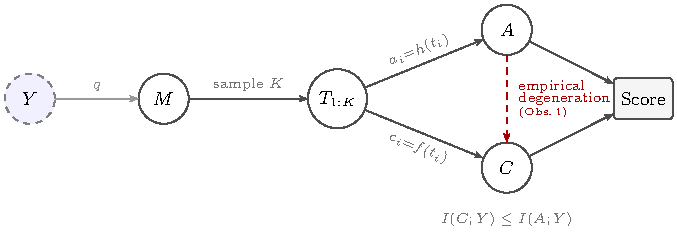
\includegraphics[width=\textwidth]{figures/fig3_causal_dag_v11.pdf}
\caption{Causal DAG of the self-extraction pipeline. Traces $T$ produce both answers $A$ and constraints $C$; under the degeneration condition (Observation~1), $C$ is empirically determined by $A$ (dashed arrow), yielding $I(C;Y) \leq I(A;Y)$. The DPI provides information-theoretic motivation; the empirical findings supply the sufficient evidence.}
\label{fig:causal-dag}
\end{figure*}

\smallskip\noindent
\textbf{Observation 1} \textit{(Argmax Preservation).}\;%
Let $t_1, \ldots, t_K \overset{\mathrm{i.i.d.}}{\sim} P_M(\cdot \mid q)$ with trace-determined answers $a_i = h(t_i)$ and $n_a = |\{i : a_i = a\}|$.
Under (i)~the degeneration condition $|\mathcal{C}^{\setminus}| \approx 0$ (Eq.~\ref{eq:degenerate}), (ii)~source-attribution scoring where $\sigma(c,a) {=} 1$ iff $c$ originates from a trace producing $a$ (Eq.~\ref{eq:score}), and (iii)~approximately uniform constraint yield per trace within each answer group, SICA reduces to majority vote: $\arg\max_a \operatorname{score}(a) = \arg\max_a n_a$.

\smallskip\noindent
\textit{Empirical support.}\;%
The degeneration condition is quantified by the Z3 rejection rate: $|\mathcal{C}^{\setminus}|/|\mathcal{C}| \approx 0.034$, confirming $|\mathcal{C}^{\setminus}| \approx 0$. Source-attribution restricts each constraint's contribution to its originating answer. For condition~(iii), per-trace constraint yield averages $5.6$--$6.0$ constraints across answer groups (median within-problem CV${=}0.26$; Appendix~\ref{app:constraint-quality}), making total weight approximately proportional to $n_a$. SICA and majority vote select the same answer on 96.1\% of problems for Qwen2.5-14B ($n{=}804$; Table~\ref{tab:ablation}) and over 90\% across all tested conditions. Varying constraint weight $\alpha$ across $[0,1]$, from pure Z3 satisfiability ($\alpha{=}0$, no source-attribution) to full source-attribution ($\alpha{=}1$), preserves ${\geq}99\%$ agreement (Table~\ref{tab:alpha-ablation}), confirming that the equivalence is driven by degeneration rather than the specific weighting scheme.

\smallskip\noindent
\textit{Per-trace separation analysis.}\;%
\looseness=-1 We directly test whether SCB is an independent bias introduced by the extraction function $f$ or a structural consequence of source-attribution scoring over correlated traces (Mistral-7B, FOLIO; 166/204 non-unanimous problems).
\emph{Extraction neutrality:} per-trace constraint density is balanced between majority and minority answer groups ($6.0$ vs.\ $5.9$ constraints/trace) and MAX-SAT exclusion rates are comparable ($0.185$ vs.\ $0.172$); $f$ produces constraints of equal quality regardless of answer group.
\emph{Formula undirectedness:} the majority of unique formulas (${\sim}$74\%) are minority-exclusive, yet most problems contain cross-group shared formulas (${\sim}$26\% of all formulas) that appear in both answer groups; under source-attribution, these shared formulas vote for each side in proportion to trace count, providing zero discriminative signal. Full semantic direction testing, evaluating each minority-trace constraint against the majority answer's truth assignment, is structurally precluded by variable isolation: 56.4\% of problems have zero variable overlap across answer groups, making cross-group satisfiability evaluation undefined.
\emph{Source-attribution as sole mechanism:} each constraint votes exclusively for its source trace's answer (by definition of source-attribution scoring). Volume amplification is ${\approx}1.0\times$; the constraint layer neither inflates nor dampens the CoT vote ratio. On 82.4\% of problems where the minority vote is correct, SICA still follows the majority (correction rate 17.6\%).
SCB is therefore a transparency property---a manifestation of CoT trace correlation \citep{kim2025correlated} complementary to but distinct from trace-level unfaithfulness \citep{turpin2023language, wan2025unveiling}: source-attribution scoring faithfully transmits the CoT trace distribution into the formal verification layer without adding or removing information. Identifying source-attribution as the mechanism (Observation~1) provides an exact locus where independence breaks, enabling the diagnostics of \S\ref{sec:diagnostic-framework} and motivating cross-architecture verification (\S\ref{sec:cross-arch}).

\looseness=-1 The Data Processing Inequality (DPI) \citep{cover2006elements} provides information-theoretic motivation: $I(C_{1:K};\, Y) \leq I(T_{1:K};\, Y)$ for any deterministic extraction $f$. The contribution is not this standard inequality but the identification of the $M{\to}T{\to}A{\to}C$ Markov chain structure in self-extraction pipelines: under the degeneration condition of Observation~1 ($|\mathcal{C}^{\setminus}| \approx 0$), constraints are fully determined by answers, yielding the tighter relationship $I(C;\, Y) \leq I(A;\, Y)$ and the approximate conditional independence $C \approx\!\!\perp Y \mid A$ (Figure~\ref{fig:causal-dag}). This provides necessary-condition reasoning, not a sufficient explanation; the empirical findings (Observation~1, BR, degeneration condition) supply the sufficient evidence.

\looseness=-1 Since the bias holds across all tested models, tasks, and extraction functions, training-free remediation strategies face a structural limitation: methods that preserve extraction accuracy necessarily inherit the model's distributional prior. This regularity holds across all 27 tested zero-shot template extraction strategies (individual results in Appendix~\ref{app:additional-interventions}); whether few-shot or iterative refinement approaches alter this pattern remains open.

\subsection{Why Remediation Fails}
\label{sec:remediation}
\label{sec:interventions}

\looseness=-1 All 27 training-free variants within the constraint-extraction paradigm, spanning four orthogonal categories (diversity, constraint-level, debate, cross-model), produce neutral-to-negative results (Figure~\ref{fig:interventions-summary}; Appendices~\ref{app:extraction}--\ref{app:entropy}). The pattern reveals a persistent independence-accuracy trade-off (Figure~\ref{fig:kappa-accuracy}). \emph{Diversity-seeking strategies} (temperature variation, persona sampling) shift $K_\text{eff}$ by $< 0.5$, insufficient to break correlation. \emph{Constraint-level interventions} (explicit negation, contrastive prompting) leave the Z3 rejection rate at ${\sim}3.4\%$; degeneration persists. \emph{Debate} ($\kappa = 0.15$, $\Delta = -18.63$\,pp) breaks correlation but collapses accuracy; \emph{cross-model extraction} achieves the lowest $\kappa$ among non-destructive methods ($\kappa{\approx}0.40$--$0.47$ vs.\ same-model $0.47$--$0.51$) but remains above the independence threshold, gaining $+0.49$\,pp (n.s.). No individual strategy achieves significance after correction (Appendix~\ref{app:intervention-individual}). Across three model families, self-extraction cannot produce constraints independent of the distributional prior.

\begin{figure}[t]
\centering
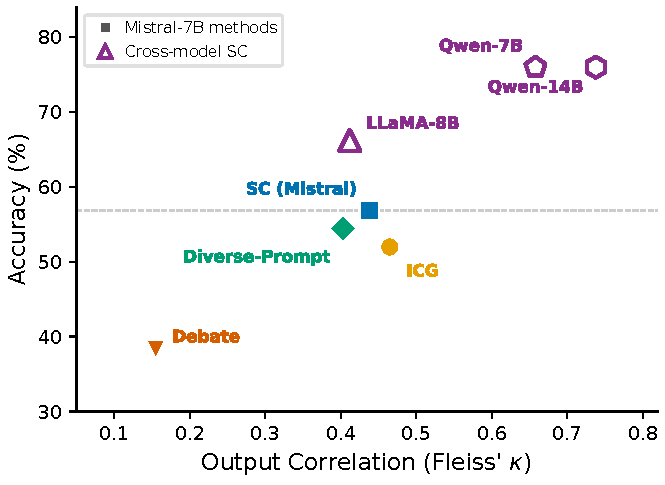
\includegraphics[width=\columnwidth]{figures/f6_kappa_accuracy_scatter}
\caption{Independence-accuracy trade-off on FOLIO ($n = 204$). Same-model methods cluster at $\kappa \approx 0.40$--$0.47$; debate breaks correlation ($\kappa = 0.15$) at catastrophic accuracy cost. Dashed line: Mistral-7B SC baseline.}
\label{fig:kappa-accuracy}
\end{figure}

\subsection{Diagnostic Framework}
\label{sec:diagnostic-framework}
\label{sec:diagnostics}

\looseness=-1 Three zero-cost diagnostics predict the outcome of any self-extraction-based aggregation from a $K{=}12$ pilot run: (1)~degenerate-regime indicator $C_0 < 5\%$ (SICA reduces to SC); (2)~diversity floor $K_\text{eff} \leq 1.30$ (insufficient vote diversity); (3)~bias ratio BR combined with SC regime (Type~A: SC $\geq 60\%$, BR $> 1$ $\to$ confirmation-bias degradation; Type~C: SC $\leq 40\%$ $\to$ error amplification). These boundaries correctly characterize failure modes across all 60 tested conditions (16 main, 27 remediation variants, 17 analytical) within the self-extraction paradigm.

\looseness=-1 Decision boundaries were derived from Mistral-7B and Qwen2.5-14B and validated prospectively on held-out generators (LLaMA-3.1-8B, Qwen3-14B), correctly predicting Type~A bias ($\Delta = -4.41$\,pp) and non-significance ($\Delta \leq +1.47$\,pp). Conversely, when diagnostics detect sufficient capability gap (\S\ref{sec:cross-arch}), the framework correctly predicts positive gain ($+6.67$\,pp for Mistral-7B on ProofWriter). The three diagnostics thus enable practitioners to rule out self-extraction pipelines before full-scale deployment.